%\pagewidth 210mm
%\pageheight 297mm
\documentclass[a4paper,10pt]{article}

\usepackage[pdfusetitle]{hyperref}
\usepackage[a4paper]{geometry}
\usepackage[bf,tiny]{titlesec}
\usepackage{fancyhdr}
\usepackage{epigraph}
%\usepackage[indent=0pt,skip=10pt]{parskip}

\usepackage{amsmath}
\usepackage{amsthm}
\newtheorem{theorem}{Theorem}
\usepackage{amssymb}
\let\mathbbalt\mathbb

\usepackage{fontspec}
\usepackage{unicode-math}
\let\mathbb\mathbbalt
%\setmainfont{TeX Gyre Termes}
%\setmathfont{TeX Gyre Termes Math}
\newcommand{\naturals}{\mathbb{N}}
\newcommand{\reals}{\mathbb{R}}
\newcommand{\rationals}{\mathbb{Q}}
\newcommand{\integers}{\mathbb{Z}}

\newcounter{problemno}
\setcounter{problemno}{1}
\newcommand{\problem}{\section*{\textbf{Problem \theproblemno}}\refstepcounter{problemno}}
\newcounter{interludeno}
\setcounter{interludeno}{1}
\newcommand{\interlude}[1]{\par\noindent\\\fbox{\begin{minipage}{\linewidth}\textbf{Interlude \theinterludeno.\enspace}#1\end{minipage}}\\\refstepcounter{interludeno}}

\newcounter{questionno}
\setcounter{questionno}{1}
\newcommand{\question}[1]{\par\noindent{\thequestionno.\enspace}#1\refstepcounter{questionno}\\}

\newcommand{\thetitle}{Some of Euler's Gems}

\renewcommand\thesection{\S{\arabic{section}}.}
\renewcommand\thesubsection{\S{\arabic{section}.\arabic{subsection}}}

\usepackage{tikz}
\usepackage{pgfplots}

\title{MEG 2023 Euler's Gems}
\author{Nathan Wong}
\date{2023}
\begin{document}
\noindent Melbourne High School\\
Maths Extension Group 2023\\
\textbf{\thetitle}\\

\begin{quote}
  \emph{Read Euler, read Euler, he is the master of us all.}
\begin{flushright}---Pierre-Simon Laplace\end{flushright}
\end{quote}

\begin{enumerate}
\item (In this problem, the famous geometric series formula
    \[ a+ar+ar^2+ar^3+\cdots+ar^{n-1}=\frac{a(r^n-1)}{r-1}\] may or may not be useful.)

  We begin by considering the charming \emph{perfect numbers}. A perfect number
  is one that is equal to the sum of its proper divisors---that is, all of its divisors including
  \(1\) but excluding itself. For example, \(6\) is a perfect number because its proper divisors
  \(1\), \(2\), and \(3\) sum to \(6\). The next perfect number is \(28\), which is \(1+2+4+7+14.\)

  Euler and Euclid proved that these numbers have something to do with \emph{Mersenne primes}. These
  are the primes of the form \(2^n-1\). For example, \(3=2^2-1\), \(7=2^3-1\), and \(31=2^5-1\) are all
  Mersenne primes.

  In terms of notation, we denote the sum of all the divisors of \(n\) (including \(n\)) as \(\sigma(n)\).
  Therefore \(\sigma(6)=1+2+3+6=12\) and \(\sigma(10)=1+2+5+10=18\). Note that \(n\) is perfect if \(\sigma(n)=2n\).
  It will also be useful to have a function \(d(n)\) that we use to denote the number of divisors of \(n\). Keeping
  with the previous examples, we have \(d(6)=d(10)=4\).
\begin{enumerate}
\item Begin by showing that if \(2^n-1\) is prime, then \(n\) is also prime. (This might not seem particularly relevant
  now, but trust that it will crop up later.)
\item Let's find out a little more about \(\sigma(n)\). As with most things in mathematics, if we know nothing
  about the properties of a function, we can only begin by plugging values in and seeing what the results are.
  In this spirit, compute the values of \(\sigma(n)\) for the first twenty values of \(n\).
\item In your table, you may notice that \[\sigma(mn)=\sigma(m)\sigma(n)\] whenever \(m\) and \(n\) are coprime.
  (A function that exhibits this property is called \emph{multiplicative}.) Out goal now is to prove this property.

  Suppose the divisors of \(m\) are \[a_1,a_2,\ldots,a_{d(m)}\] and the divisors of \(n\) are \[b_1,b_2,\ldots,b_{d(n)}.\]
  Note that this means \[\sigma(m)=a_1+a_2+\cdots+a_{d(m)}\] and \[\sigma(n)=b_1+b_2+\cdots+b_{d(n)}.\]
  
  By considering a concrete example if necessary, list the divisors of \(mn\). (Remember that \(m\) and \(n\) are coprime.)
  Hence complete the proof that \[\sigma(mn)=\sigma(m)\sigma(n).\]
\item We may also wish to find a formula for \(\sigma(n)\), a mysterious black box into which we can just plug in a number and magically
  get out the sum of its divisors. A formula does exist but for now we shall be content with proving
  that \[\sigma(p^k)=\frac{p^{k+1}-1}{p-1}\] where \(p\) is prime and \(k\) is an integer.
\item Now that we have proved the multiplicative property of the function \(\sigma(n)\) and found a formula
  for \(\sigma(p^k)\), we can turn our attention back to
  Euclid, Euler, and perfect numbers.

  The numbers connecting them are those of the form \(N=2^{p-1}(2^p-1)\) where \(2^p-1\) is prime (a Mersenne prime).
  Follow in the footsteps of the great Euclid and prove that \(N\) is perfect. That is, prove \[\sigma(N)=2N.\]
\item Now it is time for Euler to step in; he proved the converse. That is, if an even number is perfect, then it must be of
  the form \(2^{p-1}(2^p-1)\). (Interestingly, no odd perfect numbers have ever been found.)
  
  Let \(N\) be our even perfect number. Show that \(N=2^km\) for some \(k\ge 1\) and odd integer \(m\).
\item Use results we have already proved to show that
  \begin{equation}\label{eq:eulerperfect1}
  2^{k+1}m=(2^{k+1}-1)\sigma(m).
    \end{equation}
  \item Clearly \(2^{k+1}-1\) is odd. Since Equation \eqref{eq:eulerperfect1} implies that \((2^{k+1}-1)\sigma(m)\) is a multiple of \(2^{k+1}\), it
    follows that \(2^{k+1}\) must divide \(\sigma(m)\). Hence \(\sigma(m)=2^{k+1}c\) for some integer \(c\). Now show that Equation \eqref{eq:eulerperfect1}
    becomes \[m=(2^{k+1}-1)c.\]
  \item If we assume that \(c>1\), then \(m\) is divisible by at least \(1\), \(m\), and \(c\). Show that \[\sigma(m)\ge1+2^{k+1}c.\]
  \item Use the preceding inequality to derive a contradiction, and hence show that \(c=1\).
  \item Use the fact that \(c=1\) to prove that \(m\) must be prime.
  \item    We have just shown that \(m=2^{k+1}-1\) is prime. Use the first part of this problem to complete Euler's proof that every even perfect
    number is of the form \(2^{p-1}(2^p-1)\) where \(p\) and \(2^p-1\) are prime.
\end{enumerate}

\item In this problem we shall consider the fascinating infinite series \[\sum_{k=1}^{\infty}{\frac{1}{k}}=1+\frac{1}{2}+\frac{1}{3}+\frac{1}{4}\cdots\] known as the \emph{Harmonic series}.

  A few words about notation: we denote the \(n\)th partial sum of the series
  \(H_n\) and call it the \(n\)th harmonic number; that is,
  \[H_n=\sum_{k=1}^{n}\frac{1}{k}=1+\frac{1}{2}+\frac{1}{3}+\cdots+\frac{1}{n}.\]
\begin{enumerate}
\item  Our first goal is to prove that this infinite series diverges (the sum goes to infinity and doesn't converge to a finite value). Do this
  by considering consecutive terms in the sum of the form \[\cdots\frac{1}{2^k+1}+\frac{1}{2^k+2}+\cdots+\frac{1}{2^{k+1}}\cdots.\]
\item If we represent each term in the Harmonic series as the area of a rectangle with base \(1\) and height \(1/k\), we get a series
  of rectangles that look like the graph of \(f(x)=1/x\), as might be expected. This is shown in \autoref{fig:underharm}.
\begin{figure}[h]\centering
  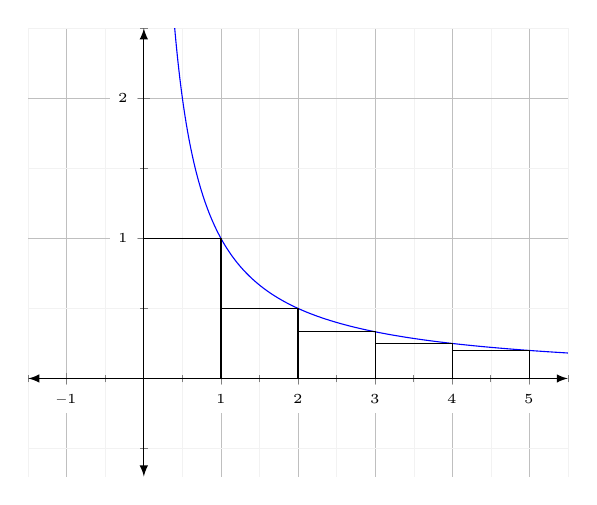
\begin{tikzpicture}
    \begin{axis}[domain=0.1:6,samples=500,
    xmin=-1,xmax=5,
    ymin=-0.2,ymax=2,
    grid=both,
    grid style={line width=.1pt, draw=gray!10},
    major grid style={line width=.2pt,draw=gray!50},
    axis lines=middle,
    minor tick num=1,
    enlargelimits={abs=0.5},
    axis line style={latex-latex},
    ticklabel style={font=\tiny,fill=white},
    xlabel style={at={(ticklabel* cs:1)},anchor=north west},
    ylabel style={at={(ticklabel* cs:1)},anchor=south west}
    ]
    \addplot+[mark=none] {1/x};
    \addplot+[mark=none,color=black] coordinates {(1,0) (1,1)};
    \addplot+[mark=none,color=black] coordinates {(2,0) (2,1/2)};
    \addplot+[mark=none,color=black] coordinates {(3,0) (3,1/3)};
    \addplot+[mark=none,color=black] coordinates {(4,0) (4,1/4)};
    \addplot[mark=none,mark options={solid},color=black] coordinates {(5,0) (5,1/5)};
    \addplot[domain=0:1] {1};
    \addplot[domain=1:2] {1/2};
    \addplot[domain=2:3] {1/3};
    \addplot[domain=3:4] {1/4};
    \addplot[domain=4:5] {1/5};
    \end{axis}
       
  \end{tikzpicture}
  \caption{A lower bound for \(\ln n\) in terms of \(H_n\)}
  \label{fig:underharm}
\end{figure}
  Note how the rectangles approximate the area under the graph of
  \(1/x\) from below. If we shift the rectangles one to the right we
  get an overestimate for the area, as shown in \autoref{fig:overharm}.
\begin{figure}[h]\centering
  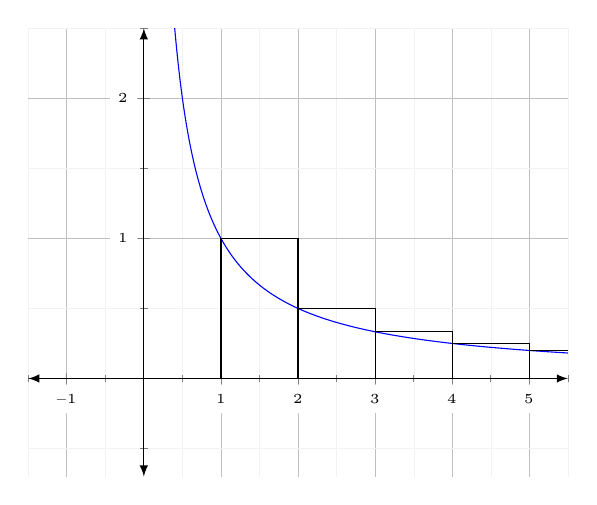
\begin{tikzpicture}
    \begin{axis}[domain=0.1:6,samples=500,
    xmin=-1,xmax=5,
    ymin=-0.2,ymax=2,
    grid=both,
    grid style={line width=.1pt, draw=gray!10},
    major grid style={line width=.2pt,draw=gray!50},
    axis lines=middle,
    minor tick num=1,
    enlargelimits={abs=0.5},
    axis line style={latex-latex},
    ticklabel style={font=\tiny,fill=white},
    xlabel style={at={(ticklabel* cs:1)},anchor=north west},
    ylabel style={at={(ticklabel* cs:1)},anchor=south west}
    ]
    \addplot+[mark=none] {1/x};
    \addplot+[mark=none,color=black] coordinates {(1,0) (1,1)};
    \addplot+[mark=none,color=black] coordinates {(2,0) (2,1)};
    \addplot+[mark=none,color=black] coordinates {(3,0) (3,1/2)};
    \addplot+[mark=none,color=black] coordinates {(4,0) (4,1/3)};
    \addplot[mark=none,color=black] coordinates {(5,0) (5,1/4)};
    \addplot[domain=1:2] {1};
    \addplot[domain=2:3] {1/2};
    \addplot[domain=3:4] {1/3};
    \addplot[domain=4:5] {1/4};
    \addplot[domain=5:6] {1/5};
    \end{axis}
  \end{tikzpicture}
  \caption{An upper bound for \(\ln n\) in terms of \(H_n\)}
  \label{fig:overharm}
\end{figure}
This overestimate is what we're interested in, since we also know
that the area under the graph of \(1/x\) starting at \(x=1\) is given by
\[\int_{1}^{x}\frac{1}{t}dt=\ln x.\]
Therefore it seems like the harmonic series approximates the natural
logarithm, with, as is evident from the diagram, some degree of error.

Using the two diagrams, show that \[\ln(n)<H_n<\ln(n)+1.\]
\item From \autoref{fig:overharm}, \(H_n\) is slightly bigger than
  \(\ln(n)\). Let's call the difference between them \(\gamma\). That is,
  \[H_n\approx \ln(n)+\gamma.\]
  Just empirically, we can see that \(\gamma\) changes depending on how large \(n\) is. \autoref{fig:table} is 
  a table showing the value of \(\gamma\) for different values of \(n\)
  (generated using Mathematica).
  \begin{figure}[h]
  \begin{center}
    \begin{tabular}{|c|c|c|c|}
      \hline
      \(n\)&\(H_n\)&\(\ln(n)\)&\(\gamma\)\\
      \hline
      \(1\)&\(1\)&\(0\)&\(1\)\\
      \(2\)&\(1.5\)&\(0.693147\)&\(0.806853\)\\
      \(3\)&\(1.83333\)&\(1.09861\)&\(0.734721\)\\
      \(4\)&\(2.08333\)&\(1.38629\)&\(0.697039\)\\
      \(5\)&\(2.28333\)&\(1.79176\)&\(0.673895\)\\
      \(6\)&\(2.45\)&\(1.79176\)&\(0.658241\)\\
      \(7\)&\(2.59286\)&\(1.94591\)&\(0.646947\)\\
      \(8\)&\(2.71786\)&\(2.07944\)&\(0.631744\)\\
      \(\vdots\)&\(\vdots\)&\(\vdots\)&\(\vdots\)\\
      \(97\)&\(5.15707\)&\(4.57471\)&\(0.583261\)\\
      \(98\)&\(5.16728\)&\(4.58497\)&\(0.582309\)\\
      \(99\)&\(5.17738\)&\(4.59512\)&\(0.582258\)\\
      \(100\)&\(5.18738\)&\(4.60517\)&\(0.582207\)\\\hline
    \end{tabular}
  \end{center}
  \caption{Table of values of \(n\), \(H_n\), \(\ln(n)\), and \(\gamma\)}
  \label{fig:table}
  \end{figure}
  We see that not only does the value of \(\gamma\) decreases as \(n\) increases, the rate of its decrease is also decreasing.
  Certainly it looks like it has a limiting value but the rate of convergence is quite slow.

  Prove that as \(n\) approaches infinity,
  \[H_{kn}-H_{n}=\ln(k)\] for any positive integer \(k\).
  Hence derive the following beautiful formulas for  natural
  logarithms.
  \begin{enumerate}
  \item 
  \[
    \ln2=1-\frac{1}{2}+\frac{1}{3}-\frac{1}{4}+\frac{1}{5}-\frac{1}{6}+\cdots.
  \]
\item
  \[
    \ln3=1+\frac{1}{2}-\frac{2}{3}+\frac{1}{4}+\frac{1}{5}-\frac{2}{6}+\frac{1}{7}+\frac{1}{8}-\frac{2}{9}+\cdots
  \]
\item
  \[
    \ln4=1+\frac{1}{2}+\frac{1}{3}-\frac{3}{4}+\frac{1}{5}+\frac{1}{6}+\frac{1}{7}-\frac{3}{8}+\cdots
  \]
  \end{enumerate}
Now try explaining why
  \[\ln n=\sum_{k=1}^{\infty}(1-n)^{1-\lceil k/n-\lfloor k/n\rfloor\rceil}\frac{1}{k}.
  \]
  (Note that \(\lfloor x\rfloor\) means the greatest integer less than or equal to \(x\) and \(\lceil x\rceil\) means the smallest integer greater than or equal to \(x\).)
\item The preceding infinite series don't really give us a way to figure
  out what \(\gamma\) is. To do that, we need some heavier mathematical
  machinery, and they don't come much heavier than the Riemann Zeta Function,
  which is defined by \[\zeta(s)=\sum_{k=1}^{\infty}\frac{1}{k^s}.\]
  This sum is quite close to the harmonic series; we get it by plugging
  in \(s=1\). Interestingly, the zeta function converges for all
  \(s>1\), which might explain why \(H_n\) diverges so slowly.

  For convenience, we define harmonic numbers \emph{of order \(r\)}
  by \[H_n^{(r)}=\sum_{k=1}^{n}\frac{1}{k^r}.\]
  This means \(H_{\infty}^{(r)}=\zeta(r)\).

  We would like to somehow use the zeta function to calculate \(\gamma\).
  How do we do this? We know \(\gamma\) is connected with the natural
  logarithm, so it makes sense to try to express a natural logarithm
  as an infinite series somewhat resembling the zeta function.

  Luckily, there is one such infinite series:
  \[\ln(1+x)=\sum_{k=1}^{\infty}(-1)^{k+1}\frac{x^k}{k}=x-\frac{x^2}{2}+\frac{x^3}{3}-\frac{x^4}{4}+\cdots.\]
  If such an infinite series looks too good to be true, derive it for yourself
  by letting \(\ln(1+x)\) be an infinite polynomial and determining the
  coefficients by comparing the higher-order derivatives of both sides at \(x=0\).
\item We see that the series has some resemblance to the zeta function,
  the biggest difference being that the powers are in the numerator. By
  introducing an appropriate substitution, show
  that
  \begin{equation}\label{eq:logkover}
    \ln\left(\frac{t}{t-1}\right)=\sum_{k=1}^{\infty}\frac{1}{kt^k}=\frac{1}{t}+\frac{1}{2t^2}+\frac{1}{3t^3}+\cdots.
  \end{equation}
  The infinite series for \(\ln(1+x)\) makes sense only when \(|x|\le 1\)
  and \(x\not=-1\). Use this to prove that Equation \eqref{eq:logkover} is defined when \(t>1\).
\item Use Equation \eqref{eq:logkover} to show that

  \begin{equation}\label{eq:lnsum} \ln(n)=(H_n-1)+\frac{1}{2}(H_n^{(2)}-1)+\frac{1}{3}(H_n^{(3)}-1)+\cdots.
  \end{equation}
\item Rearranging Equation \eqref{eq:lnsum}, we get \[
    H_n-\ln(n)=1-\frac{1}{2}(H_n^{(2)}-1)-\frac{1}{3}(H_n^{(3)}-1)-\cdots.
  \]
  This is the difference \(\gamma\) that we are looking for.
  
  As \(n\) approaches infinity, \(H_n^{(r)}\) becomes \(\zeta(r)\), so we
  can evaluate the limiting value of \(H_n-\ln(n)\):
  \[\gamma=\lim_{n\to\infty}(H_n-\ln(n))=1-\frac{1}{2}(\zeta(2)-1)-\frac{1}{3}(\zeta(3)-1)-\cdots.\]
  Using something like Mathematica or Python, calculate the
  limiting value of \(\gamma\). We have just discovered
  \emph{Euler's constant} (sometimes also called the Euler-Mascheroni constant).
  This number is very mysterious but appears in many areas of mathematics, much like
  the mathematical constants \(\pi\) and \(e\). Unlike \(\pi\) and \(e\), however,
  we are not sure if \(\gamma\) is algebraic or transcendental (whether it is the root of a polynomial
  with integer coefficients), or whether it is even
  irrational!
\item As a bonus, here's another cool thing. Since we know that
  \[H_n\approx \ln(n)+\gamma\]
  we can approximate the harmonic numbers extremely well without actually adding up all the terms in
  the series. For example, using Mathematica I get \[H_{1000}\approx7.48547\] and \[\ln(1000)+\gamma\approx7.48497.\]
  Try this for larger values of \(n\) to see how closely the natural logarithm and \(\gamma\) approximate \(H_n\).
\end{enumerate}
\item In this problem we shall consider the theory of partitions, which Euler made several contributions to. This
  theory is so rich and interesting that we only scratch the surface and consider only one of the many amazing results.
  
  A \emph{partition} of a number \(n\) is a representation of it as the sum of any number of positive
  integers. For example, the following are all the partitions of \(5\).
  \[5=4+1=3+2=3+1+1=2+2+1=2+1+1+1+1=1+1+1+1+1\]
  Think of partitions as the additive equivalent of factorisation. Unlike factorisation, however, there is no
  concept of a ``prime'', and partitions are certainly not unique, as is clearly shown in the above example.
  Note that partitions with the same numbers but different order are considered the same partition.

  In terms of notation, we denote the number of partitions of a positive number \(n\) to be \(p(n)\). Thus, for example,
  we have \(p(5)=7\).
  \begin{enumerate}
  \item Few questions about partitions can be answered from a purely combinatorial perspective. Euler managed
    to find the following generating function\footnote{A \emph{generating function} is a polynomial in which
      the coefficients are the terms of the sequence we wish to investigate. Here a generating function for the partition function
    would be a polynomial in which the coefficient of the \(x^i\) term is \(p(i)\).} for \(p(n)\):
    \begin{equation}\label{eq:pngenfunc}
      F(x)=(1+x+x^2+\cdots)(1+x^2+x^4+\cdots)(1+x^3+x^6+\cdots)\cdots.
    \end{equation}
    Describe, informally, how the coefficient of \(x^n\) in the expansion of the infinite product above is \(p(n)\).
    (If you're stuck, the partition \(10=3+2+2+2+1\) is equivalent to the term in the expanded polynomial obtained
    by choosing the \(x^3\) term in the third factor, the \(x^{6}\) in the second factor, and the \(x\) term in the first factor. Likewise,
    the partition \(5=1+1+1+1+1\) analogous to choosing the \(x^5\) term from the first factor.)
  \item Find \(p(n)\) for \(n=1,2,3,4,5,6\). What seems to be the pattern? Evaluate \(p(7)\) to see whether it continues.
  \item Show that
    \[
      F(x)=\frac{1}{(1-x)(1-x^2)(1-x^3)\cdots}.
    \]
  \item Now we begin investigating the theorem behind this problem. Let \(p_d(n)\) be the number of partitions of \(n\)
    that use distinct integers (that is, no number is used more than once in the partition).
    Find \(p_d(7)\).
  \item Let \(p_o(n)\) be the number of partitions of \(n\) that use only odd numbers (the same number is allowed to
    be used multiple times in this case). Find \(p_o(7)\).
  \item Use Equation \eqref{eq:pngenfunc} to explain why the generating function for \(p_d(n)\) is \[F_d(x)=(1+x)(1+x^2)(1+x^3)\cdots.\]
  \item Use Equation \eqref{eq:pngenfunc} to explain why generating function for \(p_o(n)\) is
    \[F_o(x)=\frac{1}{(1-x)(1-x^3)(1-x^5)\cdots}.\]
    \item Finally, complete Euler's marvellous proof that \(p_d(n)=p_o(n)\); that is, \emph{the number of partitions of a number
        into distinct numbers is equal to the number of partitions of that number into odd numbers}.
  \end{enumerate}
\end{enumerate}
\end{document}
